%!TEX encoding = UTF-8 Unicode
%!TEX root = ./../main.tex
%!TEX TS-program = xelatex

\chapter[OBP App.]{Observation Pack Approssimato} % chapter 6 title
\label{cap:sei}
L'obiettivo di questo lavoro è indagare la capacità di apprendere linguaggi regolari in uno scenario di \textit{Active Learning}, nel caso in cui non si disponga di un \textit{Oracolo} capace di rispondere nativamente ne ad \ac{EQ} ne a \ac{MQ}. La tesi è volta ad investigare lo scenario in cui si utilizzi \ac{SVM} come classificatore atto a modellare un \textit{Oracolo}, classificatore costruito a partire da alcuni esempi positivi e negativi del linguaggio da apprendere. In letteratura esistono diversi algoritmi utilizzati per  l'appredimento di linguaggi regolari. L'apprendimento di linguaggi regolari è collocabile nel più ampio tema dell' inferenza grammaticale --- usata in una varietà di campi come pattern recognition, biologia computazionale e elaborazione del linguaggio naturale --- ed è il processo di inferire automaticamente una grammatica esaminando delle stringhe di un linguaggio sconosciuto.
Il modus operandi degli algoritmi d'inferenza grammaticale o regolare  è inquadrabile all'interno dell'apprendimento per induzione e per questo è spesso detta \ac{IIR}  (o grammaticale).
Il lavoro svolto in questa tesi è volto ad approssimare un \textit{Oracolo} ed è  indipendente dallo specifico algoritmo d'\ac{IIR}, tuttavia per renderlo concreto l'attenzione è stata focalizzata sull'\ac{ObP}.
Allo stato dell'arte l' \ac{ObP} costituisce il secondo algoritmo di riferimento nell'ambito dell'apprendimento di linguaggi regolari.  L'algoritmo più performante è invece il più recente TTT algorithm \cite{SteffenTTT14}.
Si può trovare una presentazione completa dell' \ac{ObP}  in \cite{Howar12} e relativa implemetazione nella libreria LearnLib\footnote{\href{http://www.learnlib.de/}{http://www.learnlib.de/} Qui \ac{ObP} è menzionato come Discrimination Tree} .  Corredata a questa tesi vi è anche l'implementazione dell' \ac{ObP} in C++11 , codice che è stato integrato in  Gi-learning \cite{Cot16} una libreria preesistente. Nelle applicazioni reali tuttavia è altamente improbabile la disponibilità di un \textit{Oracolo} in grado di rispondere a delle \ac{EQ} da cui l'esigenza di un \textit{Oracolo ''approssimato''} la cui relativa implementazione oggetto di tesi è stata parimenti integrata in  Gi-learning \cite{Cot16}.

\section{Precedenti lavori in letteratura}
Assumere che il \textit{teacher} sia in possesso del formalismo del linguaggio target \ac{L} è uno scenario poco plausibile essendo esso stesso l'oggetto dell'inferenza.
Quindi l'obiettivo delineato in questa tesi è indagare il comportamento di un algoritmo di \textit{active learning} per inferire il \ac{DFA} A tale che $L(A) =\ac{L}$ tramite un oracolo approssimato realizzato con un classificatore statistico e tale intento si discosta dai lavori preesistenti in letteratura. In realtà una prima versione di un algoritmo di \textit{active learning} che realizza un Oracolo approssimato è già presente in Angluin \cite{Angluin87} in cui si approssima un \ac{EQ} tramite un certo numero di \ac{MQ} nella sua versione di L* approssimato. Più di recente, nella stessa direzione è andata la competizione Zulu \cite{Zulu10}: il vincitore della competizione \cite{Howar12} definisce il nuovo tipo di query: l'  \textit{Identity Query}
\begin{definizione*}[Identity Query] Testa se due prefissi $u,u'$ sono nella stessa classe di equivalenza del target A cioè se $u \not\simeq_{\lambda^{A}} \! u'$. In caso $u \not\simeq_{\lambda^{A}} \! u'$ ritorna un suffisso $v$ per il quale $\lambda^{A}(uv) \neq \lambda^{A}(u'v)$. Altrimenti ritorna il successo. 
\end{definizione*}
e dimostra che i linguaggi regolari possono essere inferiti con un numero polinomiale di \ac{MQ} ed \textit{Identity Query}.       
Le \textit{Identity Query} non sono meno realistiche delle \ac{EQ} ma forniscono un framework per organizzare le \ac{EQ} incrementalmente in modo da approssimarle in maniera relativamente facile ed efficiente tramite \ac{MQ}.  Anche gli altri algoritmi in letteratura sono focalizzati sulla ricerca di algoritmi che in maniera efficiente riescono ad approssimare le \ac{EQ} tramite \ac{MQ}.  In questa sede si assume invece l'impossibilità di rispondere nativamente anche alle \ac{MQ} oltre che alle \ac{EQ}, cioè  anche l'esito delle \ac{MQ} non è noto ed andrà approssimato.

Per quanto concerne la selezione del classificatore statistico per approssimare l'Oracolo la scelta è ricaduta su \ac{SVM} perchè costituiscono uno dei migliori modelli. Inoltre sono poche le applicazioni delle \ac{SVM} per l'apprendimento di linguaggi regolari come in \cite{Clark11}\cite{Clark06}  in cui si riesce a definire un kernel string utile per l'apprendimento dei linguaggi planari\footnote{I linguaggi planari sono una classe di linguaggi che attraversano la tassonomia di Chomsky nel senso che apprendono solo in maniera parziale i linguaggi finiti,regolari,context-free,context-sensitive ecc. senza saturare nessuno di essi}  oppure in \cite{Kontorovich09} dove si delinea un lavoro teorico sui linguaggi regolari e si propone un kernel string senza concretizzarlo specificamente per l'apprendimento di linguaggi regolari nell'accezione dell'\textit{active learning}. Altri tipi di classificatori come ad esempio le \textit{Recurrent Neural Network} si sono rilevate particolarmente adatte allo scopo di modellare un \ac{DFA} ma come si evince da \cite{Forcada02}, che costituisce una panoramica su di esse a riguardo dell'impiego in  \ac{GI}, sono state già ampiamente dibattute in letteratura.

\section{Funzionamento ObPA}

\section{Generazione di campioni da un DFA}
\label{sec:gensam}
La valutazione delle \textit{performances} di un algoritmo di \ac{GI} possono essere influenzate sia positivamente che negativamente da alcuni fattori \cite{Stamina10}: 
\begin{itemize}
\item Numero di campioni del \textit{training set} e del \textit{test set}
\item campioni suddetti strutturalmente completi
\item Complessità del \ac{DFA} target 
\end{itemize}

Se si decidesse di generare  i campioni come stringhe casuali fino a una certa lunghezza in cui ogni simbolo costituente una stringa è estratto in maniera uniforme tra tutti i simboli dell'alfabeto si  incorrerebbe nel problema che  si verrebbe ad avere un insieme non bilanciato a causa della predominanza di campioni negativi dato che tipicamente su $\Sigma*$ sono in minoranza le stringhe accettate da un \ac{DFA}. 
Inoltre  per l'addestramento di un classificatore e anche per un algoritmo di \ac{GI} è molto importante avere un insieme caratteristico (definizione \label{def:car}) o perlomeno un insieme di stringhe che raggiunge gran parte degli stati e delle transizioni di un \ac{DFA}.
In \cite{Stamina10} è descritto un algoritmo in grado di assicurare con altà probabilità la completezza strutturale dei campioni e di produrre campioni bilanciati. L'algoritmo effettua un \textbf{random walk} sul \ac{DFA} target e si rimanda al riferimento per i dettagli.
La proprietà dei campioni di essere strutturalmente completi(c'è solo una probabilità alta che lo siano ma non la certezza) potrebbe condurre a delle stime ottimisticamente biased dell'algoritmo \ac{ObPA} dato che i campioni a disposizione dell'utente sono di norma del tutto casuali (anche con random walk lo sono ma come detto in modo da esplorare tutti i percorsi del \ac{DFA})  . Nonostante ciò si è deciso  di utilizzare comunque \textit{random walk}  perchè  questa procedura è diventata uno standard de facto per generare i campioni nelle competizioni tra algoritmi riguardanti \ac{GI}.

\subsection{W-Method}
Per la generazione di un \textit{test set} per fare model evaluation  è improbabile che delle stringhe generate casualmente testino adeguatamente un classificatore. Quindi per la generazione del \textit{test set} dacade la valenza del discorso che campioni strutturalmente completi potrebbero condurre a sovrastimare positivamente un classificatore, assunto che rimane valido per il \textit{training set}, ma il possedimento di questa proprietà dei dati nel \textit{test set} è ricercata per testare in maniera affidabile un classificatore che difatti approssima \ac{L}. Quindi l'utilizzo di \textit{random walk} per la generazione del \textit{test set} è assolutamente appropriato.    \ac{ObPA} però necessita anche del confronto dell'ipotesi intermedia \ac{H} ottenuta ad ogni \textit{round} con il \ac{DFA} target ma quest ultimo non è noto ma è approssimato da un classificatore\footnote{il classificatore approssima l'Oracolo, ma in ultima istanza ad essere approsimato è linguaggio alias \ac{DFA} target dato che un Oracolo nel caso ideale ha il \ac{DFA} target e tramite esso risponde alle query} preliminarmente costruito tramite \ac{SVM} a partire dai campioni disponibili.   Di conseguenza l'\ac{EQ} come spiegato in [INSERIRE RIFERIMENTO SEZIONE] va implementata sottoponendo  una serie di stringhe sia al classificatore che al \ac{DFA} ipotesi \ac{H} ed è fondamentale che queste stringhe siano selezionate in maniera attenta. Estrarre le stringhe con l'algoritmo \textit{random walk} sul \ac{DFA} target in questo caso genera delle stringhe particolarmente significative ma solo per il \ac{DFA} \ac{H} ma possibilmente non rappresentative del \ac{DFA} target dato che è ignoto.\\
 E ancora sia  \textit{random smapling} che \textit{random walk} possono produrre un \textit{test set} che ha alcuni campioni in comune con il \textit{training set} con cui è stato addestrato il classificatore che approssima l'oracolo ottenendo una possibile corrispondenza mistificatoria dell' \ac{EQ}.\\
 Inoltre solo per la \textit{debug version} è possibile confrontare il \ac{DFA} finale inferito da \ac{ObPA} con il \ac{DFA} target ed anche in questo caso si ripresentano i problemi precedentemente esposti cioè eseguendo \textit{random walk} su uno dei due automi (o il target o l'ipotesi) potrebbe essere prodotto un insieme di stringhe per testare la similarità dei due linguaggi che non esplora parte dell'altro \ac{DFA} (quello su cui non si è eseguito \textit{random walk}) risultando quindi non del tutto appropriato allo scopo. Pertanto adesso è descritto l' algoritmo \textbf{W-Method} non affetto dai problemi summenzionati

\subsubsection{Algoritmo W-Method}
Tramite il W-Method nel contesto della \ac{GI} si realizza un' \ac{EQ} esatta impiegando solo \ac{MQ} \cite{Balanescu03}. Infatti esso crea, senza la necessità di avere il \ac{DFA} target A,  un \textit{test set}  $X$ dall'ipotesi \ac{H} in modo che se $\forall x \in X \:\:\: \lambda^{A}(x) = \lambda^{H}(x) \text{allora} A \cong \ac{H}$  (per rispondere alle \ac{MQ} lato target non è strettamente necessario avere il \ac{DFA} target ma si suppone uno scenario in cui si possa conoscere l'esito di $\lambda^{A}(x)$ senza la sua conoscenza ). Quindi il W-Method si può usare per realizzare un'\ac{EQ} in maniera esatta tramite \ac{MQ} tuttavia il numero di stringhe generate dal \textit{W-Method} può essere enorme e quindi subentrano problemi di efficienza. In questa tesi è incognito anche l'esito delle \ac{MQ} che è approssimato tramite le \ac{SVM} quindi l'\ac{EQ} realizzata tramite il \textit{W-Method} sarà comunque un'approsimazione. Inoltre quanto detto è vero se verificate alcune condizioni tra cui il numero esatto di stati del \ac{DFA} target   che in \ac{ObPA} non è noto nella \textit{release version} e può essere solo stimato producendo quindi un insieme di stringhe che approssimano l'equivalenza senza garantirla. Gli altri requisiti del \textit{W-Method} sono \cite{Balanescu03}:
\begin{itemize}
\item \ac{H} ed A sono deterministici
\item \ac{H} è canonico
\item Non ci sono stati irraggiungibili nè in \ac{H} nè in A
\item Si conosce $\norma{A}$
\item \ac{H} e A devono essere completamente specificati cioè da ogni stato per ogni $\Sigma$ si raggiunge uno stato che non sia lo stato pozzo(questa condizione può essere rilassata \cite{Balanescu03})
\end{itemize}
Si descrive brevemente il W-Method a grandi linee.   La ratio è che nel target potrei avere degli extra-stati che non vengono esplorati con il \textit{test set} generato con metodi classici e che potrebbero causare un comportamento indesiderato ed alterare la valutazione senza averne avvisaglie. Per questo motivo si stima in anticipo in numero di stati nel \ac{DFA} target (in modo che il test set esplori tutti gli stati del target). Per questo motivo è importante eseguire il \textit{W-Method} sul \ac{DFA} (tra ipotesi e target quando in \textit{debug version} si testa la similarità tra il target ed \ac{H}) che ha il numero minore di stati stimando gli stati dell'altro.\\
Ipotizzando in chiave espositiva che il \ac{DFA} col numero minore di stati sia \ac{H} si procede generando lo \textit{state cover} $C$ su \ac{H} cioè  $C =\{c : \forall q \in Q^{\ac{H}} \:\: \hat{\delta}^{\ac{H}}(q_\epsilon,c)=q\}$ cioè l'insieme di stringhe necessarie per raggiungere ogni stato a partire dallo stato iniziale. Due stati $q_1,q_2$ di \ac{H} sono detti \textit{W-distinguibili} se dato un insieme di stringhe $W \subseteq \Sigma^{*}  \: \:\exists x \in W : ( ( \lambda^{\ac{H}}_{q_{1}}(x) = 1 \land \lambda^{\ac{H}}_{q_{2}}(x) = 0) \lor ( \lambda^{\ac{H}}_{q_{1}}(x) = 0 \land \lambda^{\ac{H}}_{q_{2}}(x) = 1) )$ . W è detto un \textit{characterization set} se tutti gli stati distinti di \ac{H} (essendo \ac{H} minimo tutti gli stati sono distinti) presi a due a due  sono \textit{W-distinguibili}. Definito $k = \norma{A} - \norma{H}$ essere una stima (si parla di stima perchè il target A è ignoto) di quanti stati ha il target in più dell'ipotesi si ha che il \textit{test set} $Y$ è:
\begin{equation*}
Y = C(\{\epsilon\} \cup \Sigma \cup \dots \cup \Sigma^{k+1})W
\end{equation*}

Il difetto di questa tecnica è che la complessità dipende in maniera esponenziale [VEDI CHOW pag.181] da  $\norma{A} - \norma{H}$ e quando questa differenza di stati diventa grande il metodo è ingestibile e il numero di stringhe generate dal \textit{W-Method} diventa enorme.




\section{ALtro}
Inserire il discorso che in debug version alla fine è comunque necessario confrontare l'ipotesi finale col target per rendersi conto del dfa inferito quanto è buono. Infatti che l'ipotesi sia verificato tramite un'equivalence query essere simile al classificatore non è sufficiente in quanto il classificatore è già di per sè un'approssimazione del target e quindi un'ipotesi che approssima bene il classificatore potrebbe non approssimare bene il target e quindi un confronto finale tra target e ipotesi è necessario. 




\section{Scelte Progettuali}
Un lavoro d'implementazione degno di nota è costituito dalla preliminare ingegnerizzazione del codice. Come detto il prescelto algoritmo di \textit{active learning} è stato \ac{ObP}, che nella sua versione base presentata nel capitolo \ref{cap:quattro} necessita di un \ac{DFA} target che funge da Oracolo onnisciente. Nell'ottica di preservare questa versione dell'\ac{ObP} e contemporaneamente integrare nella libreria le funzionalità dell'\ac{ObPA} si è deciso di implementare una versione polimorfica. Più in dettaglio si è creata una gerarchia di classi per l'entità astratta Oracolo come in figura \ref{fig:eor}.
\begin{figure}[htp]
	\centering
	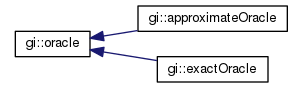
\includegraphics[ width=0.7\textwidth]{EreditaOracolo}
	\caption[Ereditarietà Oracolo]{Ereditarietà Oracolo}
   \label{fig:eor}
\end{figure}

L'algoritmo \ac{ObP} invece di possedere (composizione) un \ac{DFA} target ha un oggetto della classe base astratta Oracolo. Quando invoco il costruttore dell' \ac{ObP}  si deve passare anche l'indirizzo di un oggetto della classe Oracolo. Tramite il tipo di oggetto Oracolo(si ha un handle della classe base Oracolo che punta allo specifico oggetto della classe derivata passato) passato  viene determinato in maniera trasparente con il polimorfismo se si desidera utilizzare l'\ac{ObP} piuttosto che l'\ac{ObPA}. Le chiamate alle funzioni effettuate sull'oggetto Oracolo all'interno di \ac{ObP} hanno la stessa \textit{signature} , cioè le \ac{MQ} e le \ac{EQ} , ma il tipo dell'oggetto Oracolo passato determina automaticamente di quale classe derivata invocare le funzioni (che avranno diverse implementazioni a secondo se appartengono alla classe exactOracle o a quella approximateOracle).  In questo modo la classe dell'algoritmo \ac{ObP} ha subito pochissime modifiche  e il lavoro d'implementazione di questa tesi si è focalizzato sulla classe approximateOracle. Infine all'interno della classe observation\_pack , per impedire al \textit{client} di vedere le strutture dati e le modifiche effettuate su di esse  e in ultimo il modo in cui funziona l'algoritmo, è necessario effettuare una copia interna dell'Oracolo passato dal \textit{client} ma non conoscendo a priori di quale tipo, e quindi di quale classe, è l'Oracolo vi è stata la difficoltà su come invocare il costruttore di copia. A tal fine si è usata la tecnica del \textit{clone idiom} .Quando si ha un riferimento polimorfico cioè un 
  puntatore alla classe base che punta a un oggetto della classe derivata all'occorrenza può sorgere il problema di determinare qual è il tipo della classe derivata . Allora nella classe base si dichiara un metodo virtuale puro che tutte le classi derivate devono quindi implementare. Quest'implementazione consiste nella creazione dinamica  di un nuovo oggetto della classe derivata chiamando il costruttore di copia della classe derivata sull'oggetto corrente (tramite new classeDerivata(*this)). Questo nuovo oggetto creato verrà tornato al chiamante. Si noti che il costruttore di copia della classe derivata deve provvedere a chiamare il costruttore di copia della classe base e che in questi costruttori deve avvenire una deep copy di tutti i membri dinamici.   In figura \ref{fig:cba} l'interfaccia della classe base astratta.
  
 \begin{figure}[htp]
	\centering
	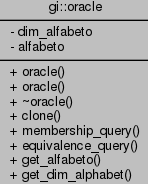
\includegraphics[ width=0.3\textwidth]{Oracolo}
	\caption[Interfaccia classe base Oracolo]{Interfaccia classe base Oracolo}
   \label{fig:cba}
\end{figure}    